\setcounter{chapter}{-1} % sets the number of this chapter to 0
\chapter{About Latex and this Template}

This is the official template for the chair of computer graphics and visualization.  It is based on the TU corporate design, more exactly on the \texttt{tudscrbook} class, which is a wrapper for the \texttt{scrbook} Koma script. The documentation\footnote{\href{https://ftp.tu-chemnitz.de/pub/tex/macros/latex/contrib/tudscr/doc/tudscr.pdf}{https://ftp.tu-chemnitz.de/pub/tex/macros/latex/contrib/tudscr/doc/tudscr.pdf}} of the wrapper class might be useful, if there are things you need to understand and are not covered in this short description.

\section{Using the Template}
This template comes with a few files. This section will guide you through their structure, but will also explain, how to switch languages and how to change the type of your work.

\subsection{File Structure}
The multiple files of this template contain the different parts of the work. They are all brought together by the \texttt{main.tex} file, which solely purpose is, to connect all the files as the \emph{root document}. When you are using Texmaker or TeXStudio to edit and compile these files, you should apply the option to make this file the \emph{root document}.

All other text files are contained within four folders:
\vspace{-\topsep} % removes the addiotional line between the sentence and the list
\begin{itemize}
	\item \textbf{0\_frontmatter:} Contains all files that are technically needed to define the documents properties and formal pages such as the \emph{"Statement of Authorship} as well, as all other parts of the work, which are placed before the actual chapters of the work.
	\item \textbf{1\_mainmatter:} Contains the chapters of the work
	\item \textbf{2\_bib:} Contains the bib-file, as well as a tex file to print the bibliography within the document. It is possible to use multiple bib-files, just make sure every file is added in the \emph{header} with \texttt{\textbackslash addbibresource\{path to file\}}.
	\item  \textbf{3\_appendix:} Contains any appendix files, in the template, there is only an example file with some blind text.
\end{itemize}

There are two additional folders:
\vspace{-\topsep}
\begin{itemize}
	\item \textbf{fig:} For image files.
	\item \textbf{logo:} Containing the logos of the chair.
\end{itemize}

Within the frontmatter-directory, there are the following files:
\vspace{-\topsep}
\begin{itemize}
	\item \textbf{0\_header:} Containing the definition of the used class, as well as most parameters and used packages.
	\item \textbf{1\_title:} Defines the information used for creating the title. It is also used to define some pdf meta data. The subject of the work is also defined in this file. All possible subjects can be found in the documentation.
	\item \textbf{2\_task:} A file used to include the task description.
	\item \textbf{3\_declaration:} Adds the statement of authorship.
	\item \textbf{4\_abstract:} Side containing an English and a German abstract.
	\item \textbf{5\_acronyms:} The place to declare your used acronyms.
\end{itemize}


\subsection{Changing the Language to German}
The standard language for this template is English. However, everything needed for changing the language to German is already in the template. To do this, enter the \texttt{0\_frontmatter/0\_header.tex} file and search the first few lines of the document for \texttt{ngerman, english,} in the \texttt{documentclass} options. Then swap the order to \texttt{english, ngerman,}. You still have to translate some of the text, but most things should change into German automatically.


\subsection{Biblatex and Biber}
This template uses \texttt{biblatex} and \texttt{biber} for creating a bibliography. However, most editors use the older \texttt{bibtex} as a standard\footnote{A discussion of the differences of both bibliography tools and the problems one or the other may cause can be found here: \url{https://tex.stackexchange.com/questions/25701/}}. To change this in TeXStudio or Texmaker, just enter Options -> Configure TeXStudio/Texmaker -> Build and change the default bibliography tool from bibtex to Biber. You can also just change the bibliography back to bibtex in the \emph{0\_frontmatter/0\_header.tex} file by replacing the \texttt{backend=biber} option for the \texttt{biblatex} package back to \texttt{bibtex}.
Most scientific resources allow to export a bibtex-citation directly, which can be copied to the bib file and used with the \texttt{\textbackslash cite\{<identifier>\}} command. The result should look like this: \cite{Foley1982}.

\subsection{Adapt the Template to Different Types of Works}
When writing a diploma, bachelor's or master's thesis, there is little to change in this template. The \texttt{\textbackslash{}subject{}}-field in the title page, see Table \ref{tab:subj-id} for possible values, and the \texttt{\textbackslash{}graduation[<short form>]{<degree>}}-field in the \texttt{0\_frontmatter/1\_title.tex} need to be adjusted. For other works, the task-description and declaration of independence should be removed by deleting the lines referencing the files \texttt{2\_task.tex} and \texttt{3\_declaration.tex} in the \texttt{main.tex} file, the list of figures and the list of tables could also be removed there. When the work is never intended to be printed, it might also be a consideration to change some of the options for the \texttt{\textbackslash{}documentclass} in the \texttt{0\_frontmatter/0\_header.tex}. Expecially there is no need for additional space at the inside, so the \texttt{bcor}-parameter, used to compensate the print area in respect to the book thickness when printed, can be set to zero or removed completely and the \texttt{twoside}-parameter with the following outside paging might be irritating and can be changed to \texttt{oneside}.

\begin{table}[t]
	\centering
	\caption{All possible types of work.}
	\label{tab:subj-id}
	\renewcommand{\arraystretch}{1.3}
	\begin{tabular}{@{}llll@{}}
		\toprule
		Value          & German            & English                  \\ \midrule
		diss           & Dissertation      & Dissertation             \\
		doctoral       & Dissertation      & Dissertation             \\
		phd            & Dissertation      & Dissertation             \\
		diploma        & Diplomarbeit      & Diploma Thesis           \\
		master         & Master-Arbeit     & Master Thesis            \\
		bachelor       & Bachelor-Arbeit   & Bachelor Thesis          \\
		student        & Studienarbeit     & Student Thesis           \\
		evidence       & Großer Beleg      & Student Research Project \\
		project        & Projektarbeit     & Project Paper            \\
		seminar        & Seminararbeit     & Seminar Paper            \\
		term           & Hausarbeit        & Term Paper               \\
		research       & Forschungsbericht & Research Report          \\
		log            & Protokoll         & Log                      \\
		report         & Bericht           & Report                   \\
		internship     & Praktikumsbericht & Internship Report        \\ \bottomrule
	\end{tabular}
\end{table}

\section{Latex Basics}
The following sections will explain some of  the Latex basics. It is especially concerned with figures (\ref{texbas:fig}), acronyms (\ref{texbas:acr}), equations (\ref{texbas:eq}), tables (\ref{texbas:tab}) and code listings (\ref{texbas:code}). If you already worked with Latex, there is probably no need to read this, but if you never used Latex or are stumbling over some of the elements in this template, it might be useful. It shows also some of the notations used at the \ac{CGV lab}, so looking in the source code of this file (\texttt{1\_mainmatter/0\_about\_this\_template.tex}) might be useful.

\subsection{Weblinks}
For Weblinks there are two ways to include them into a latex document. You can just use the \texttt{\textbackslash url\{<url>\}} command or use \texttt{\textbackslash href\{<url>\}\{<text>\}}.
While an example link with the \texttt{url} command would look like \url{https://wwwpub.zih.tu-dresden.de/~gumhold/cgv/html/overview.html}, href is probably a more elegant solution, where the \href{https://wwwpub.zih.tu-dresden.de/~gumhold/cgv/html/overview.html}{link to the cgv framework on pub.zih.tu-dresden.de} can be embedded into the text. However, as long as the link color is black (which it should be for printed formats), the link is hard to find and in a printed format, the information about the link is lost entirely, if it is not contained within the text. So writing down at least a part of the link can help with recognizing the link as a link. Links should not be placed in the text, but rather in footnotes using the \texttt{\textbackslash footnote\{footnote\}}-command. 

\subsection{Figures}
\label{texbas:fig}
You can embed figures with the commands shown in figure \ref{fig:code_for_fig}. The result for an example should look like figure \ref{fig:Stanf_Bunny}. Figure objects are useful to include graphics, but can also host a range of other elements. The most important property of figures is, that they are floating objects, which latex is trying to place where they fit best.

\begin{figure}[ht]
	\begin{lstlisting}[language=TeX]
\begin{figure}[ht] 		% [h] tries to keep the figure [h]ere, [t]op is used as alternative
	\centering		% center the graphic, if it is smaller then the page
	\includegraphics[width=<scaling factor>\textwidth]{<path to the graphic>}
	\caption{<The text to describe the graphic.>}
	\label{<A label to refer to the graphic in the text.>}
\end{figure}	
	\end{lstlisting}
	\caption{Code for embedding graphics}
	\label{fig:code_for_fig}
\end{figure}

\begin{figure}[ht]
	\centering
	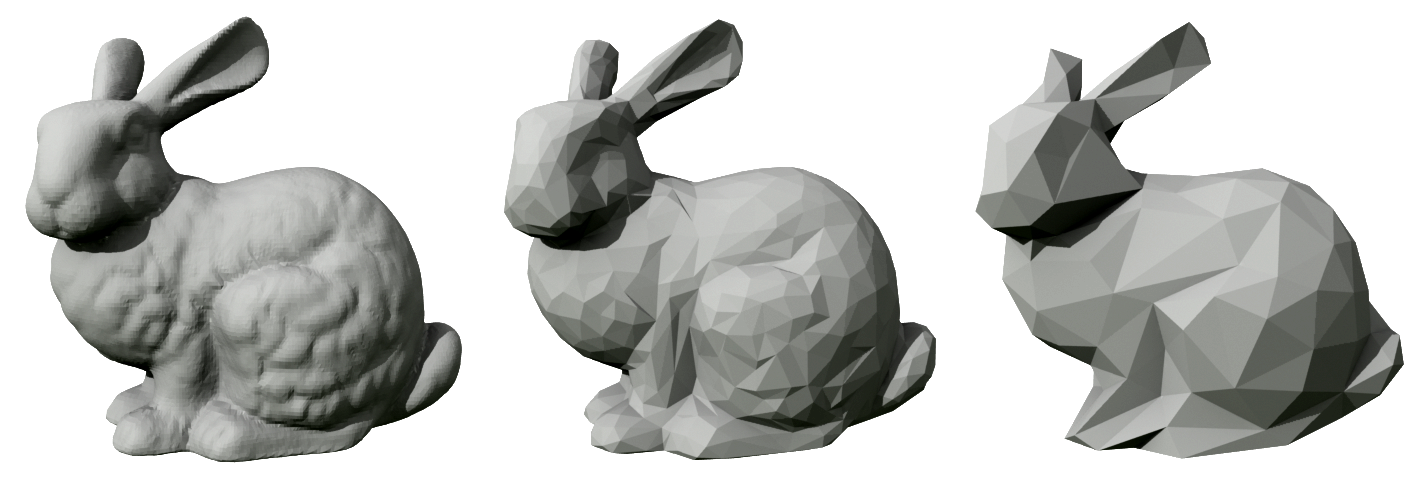
\includegraphics[width=1\textwidth]{fig/Stanford_bunny_qem.png}
	\caption{Quadric error metric simplification applied to the Stanford bunny}
	\label{fig:Stanf_Bunny}
\end{figure}

\subsection{Symbols and Acronyms}
\label{texbas:acr}
This template uses the \emph{acronyms}-package to include a list of symbols and acronyms at the beginning of the work. Acronyms can be referenced with the \texttt{\textbackslash ac\{<identifier>\}} command. E.g. using \texttt{\textbackslash ac\{GPU\}} in this document results in: \ac{GPU}, the name of the acronym or symbol, as well as the acronym or symbol itself in brackets. After the first use, only the acronym or symbol will be used. The \texttt{acronyms}-package will throw a warning if an acronym is not used within the work.


\subsection{Equations}
\label{texbas:eq}
Equations can be used with the math environment, which can be delimited either inline by using the \$ eq \$, \texttt{\textbackslash [ eq \textbackslash ]}, or separated from the text with \texttt{\textbackslash begin\{equation\} eq \textbackslash end\{equation\}}. The latter will additionally enumerate the equation and allows for a label, so we can reference an equation like the equation \ref{eq:example}.


\begin{equation}
	 x^n + y^n = z^n
	\label{eq:example}
\end{equation}

You can also place equations within a figure. The equation then becomes a floating object and might be placed somewhere else, but can also be captioned, as equation \ref{eq:pythagorean} in figure \ref{fig:pythagorean}. However, having an equation start with \emph{"Figure"} is not always optimal. The German "Abbildung" is even worse.

\begin{figure}[hb]
	\begin{equation}
		x^2 + y^2 = z^2
		\label{eq:pythagorean}
	\end{equation}
	\caption{Pythagorean Theorem}
	\label{fig:pythagorean}
\end{figure}

\subsection*{CGV specific notation and symbols}

In CG we work with 2D, 3D and 4D vectors $v \in \mathbb{R}^d$. Vectors can represent different entities. At the \ac{CGV lab}, we use the notation shown in figure \ref{fig:eq_ex} for them. All the notations can also be looked up in the slides of the cg-courses.

\begin{figure}[t]
	\centering
	\begin{subfigure}[t]{0.4\textwidth}
			\centering
			\large
			\begin{bfseries}
			\textcolor{cddarkblue}{Directions} \\
			\end{bfseries}
			\normalsize
			\smallskip
			
\includegraphics[width=1cm]{fig/vec.png} \\
			\smallskip
			
			$\bm{\vec{d}} \in \mathbb{R}^d$
	
			\begin{bfseries}
				\textcolor{cddarkblue}{Normals} \\
			\end{bfseries}
			\normalsize
			of length 1
			
			$\bm{\hat{n}} \in \mathbb{R}^d$	
	\end{subfigure}
	{\color{gray!10}\vrule}
	\begin{subfigure}[t]{0.4\textwidth}
			\centering
			\large
			\begin{bfseries}
				\textcolor{cddarkblue}{Positions} \\
			\end{bfseries}
			\normalsize
			\medskip
			
\includegraphics[width=0.3cm]{fig/pos.png}
			\medskip
			
			$\bm{\underline{p}} \in \textup{A}^d$
	\end{subfigure}
	
	\bigskip
 	{\color{gray!10}\hrule}
 	\bigskip

	\begin{subfigure}[t]{0.4\textwidth}
			\centering
			\large
			\begin{bfseries}
				\textcolor{cddarkblue}{Planes} \\
			\end{bfseries}
			\normalsize
			\smallskip
			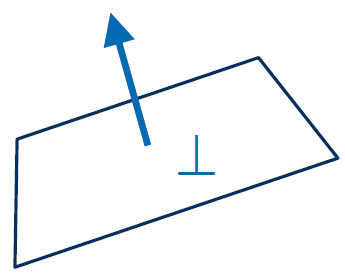
\includegraphics[width=2cm]{fig/plane.png} \\
			\smallskip
			$\bm{n}=\begin{pmatrix} n_x\\ n_y\\ n_z \\ d \end{pmatrix} \rightarrow \bm{n^Tx} = 0 $
	\end{subfigure}
	{\color{gray!10}\vrule}
	\begin{subfigure}[t]{0.4\textwidth}
			\centering
			\large
			\begin{bfseries}
				\textcolor{cddarkblue}{Colors} \\
			\end{bfseries}
			\normalsize
			\smallskip
			
\includegraphics[width=2cm]{fig/col.png} \\
			\smallskip
			$\bm{\dddot{c}} \in \bm{\dddot{C}}$
	\end{subfigure}
	
	\bigskip
	{\color{gray!10}\hrule}
	\bigskip
	
	\begin{subfigure}{0.4\textwidth}
		\centering
		\large
		\begin{bfseries}
			\textcolor{cddarkblue}{Unified Representation \\ of Positions} \\
		\end{bfseries}
		\footnotesize
		by using an additional w component	\\	
		$\bm{\underline{p}}=\begin{pmatrix} x\\ y\\ z \end{pmatrix} \rightarrow \bm{\widetilde{p}} = \begin{pmatrix} x\\ y\\ z \\ 1 \end{pmatrix} $

		
		1 denotes a position
	\end{subfigure}
	{\color{gray!10}\vrule}
	\begin{subfigure}{0.4\textwidth}
		\centering
		\large
		\begin{bfseries}
			\textcolor{cddarkblue}{Unified Representation \\ of Directions} \\
		\end{bfseries}
		\footnotesize
		by using an additional w component		\\
		$\bm{\vec{d}}=\begin{pmatrix} x\\ y\\ z \end{pmatrix} \rightarrow \bm{\widetilde{d}} = \begin{pmatrix} x\\ y\\ z \\ 0 \end{pmatrix} $
		
		0 denotes a direction.
	\end{subfigure}

\caption{Some of the different notations for multiple types of vectors. All the notation types can be looked up in the computer graphics lecture slides.}
\label{fig:eq_ex}
\end{figure}


\subsection{Tables}
\label{texbas:tab}
In Latex, tables are generated using the tabular environment.
As this is often far more complicated then in editors following the \emph{\ac{WYSIWYG}} principle, a tool for building tables in a \ac{WYSIWYG} manner and translating them to Latex-Code can be useful.
Examples for such tools are latex-tables.com\footnote{\url{https://www.latex-tables.com/}} and tablesgenerator.com\footnote{\url{https://www.tablesgenerator.com/}}.
When creating tables, there should generally be no vertical lines and only three horizontal lines\footnote{A neat little guide on how to make tables look nice can be found here: \url{https://people.inf.ethz.ch/markusp/teaching/guides/guide-tables.pdf}}\footnote{Another helpful source about tables might be this blog post by Nick Higham: \url{https://nhigham.com/2019/11/19/better-latex-tables-with-booktabs/}}.
A table in latex might look like table \ref{tab:example}. The code for creating this table can be found in the code box \ref{fig:code_for_tab}. Please note: In contrast to figures, tables must have the caption above the content and also and also should be placed at the top of a page, which is achievable by using the placement parameter \texttt{[t]}. For very long tables, the \texttt{longtable}-package\footnote{For reading even more about tables and the possible packages, this wikibooks entry could be interesting: \url{https://en.wikibooks.org/wiki/LaTeX/Tables}} might help with its support for tables spanning multiple pages. 

\begin{table}[t!]
	\centering
	\caption[Average absolute error for the implementations]{Average absolute error in slices and percentage, by size of implementation. This table is from a paper from Milder et al. \cite{Milder2006}.}
	\renewcommand{\arraystretch}{1.3}
	\begin{tabular}{@{}rrrcrr@{}}\toprule
		\multicolumn{1}{l}{slices} & \multicolumn{2}{c}{abs. Error (\%)} & \phantom{abc}& \multicolumn{2}{c}{abs. Error (slices)}\\
		\cmidrule{2-3} \cmidrule{5-6}
		& avg. 	& max. 	&& avg.	& max.	\\ \midrule
		<5000 		& 7.4	& 75.0 	&& 118 	& 835	\\
		5000-10000 	& 2.4	& 14.4	&& 162	& 756	\\
		10000-15000 & 2.0	& 11.5	&& 232	& 1235	\\
		>15000		& 2.3	& 14.5	&& 438	& 2287	\\
		\bottomrule
	\end{tabular}
	\label{tab:example}
\end{table}

\begin{figure}[t!]
	\begin{lstlisting}[language=TeX]
\begin{table}[t]
	\centering
	\caption{Average absolute error in slices and percentage, by size of implementation. This table is from a paper from Milder et al. \cite{Milder2006}.}
	\renewcommand{\arraystretch}{1.3}
	\begin{tabular}{@{}rrrcrrc@{}}\toprule
		\multicolumn{1}{l}{slices} & \multicolumn{2}{c}{abs. Error (\\%)} & \phantom{abc}&
		\multicolumn{2}{c}{abs. Error (slices)}\\
		\cmidrule{2-3} \cmidrule{5-6}
				& avg. 	& max. 	&& avg.	& max 	\\ \midrule
		<5000 		& 7.4	& 75.0 	&& 118 	& 835	\\
		5000-10000 	& 2.4	& 14.4	&& 162	& 756	\\
		10000-15000 & 2.0	& 11.5	&& 232	& 1235	\\
		>15000		& 2.3	& 14.5	&& 438	& 2287	\\
		\bottomrule
	\end{tabular}
	\label{tab:example}
\end{table}

	\end{lstlisting}
	\caption{Code for the example table \ref{tab:example}}
	\label{fig:code_for_tab}
\end{figure}


\subsection{Code}
\label{texbas:code}
With the \texttt{lstlisting} environment you can show code. The most important difference to normal text is, that spaces and tabs are kept in place within that environment and Latex commands will not be executed. You can however escape latex commands with the [escapeinside={}{}]\footnote{Here is an example on how to do that: \url{https://tex.stackexchange.com/questions/63729/}} option. An example for how to show code can be seen in \ref{fig:code_for_code}, which results in \ref{code:example}.

\lstnewenvironment{TeXlstlisting}{\lstset{language=[LaTeX]TeX}}{}
\begin{figure}[ht]
	\begin{TeXlstlisting}
\begin{figure}[htbp]
	\begin{lstlisting}
//comment
for(int i = 0; i < 100;i++)
{
	test(i);
}
	\end{lstlisting}
	\caption{Example for a code block.}
	\label{code:example}
\end{figure}
	\end{TeXlstlisting}
	\caption[Code for showing code.]{Code for showing the code block below. As tabs are preserved in listings, there should be no tabs in the code, that you do not want to see in the output.}
	\label{fig:code_for_code}
\end{figure}

\begin{figure}[ht]
	\begin{lstlisting}
//comment
for(int i = 0; i < 100;i++)
{
	test(i);
}
	\end{lstlisting}
	\caption{Example for a code block.}
	\label{code:example}
\end{figure}

